\documentclass[12pt]{article}
\usepackage[utf8]{inputenc}
\usepackage{gaml}

% refer to configurations.tex for the LaTeX setup of this template
\usepackage[english]{babel}

\title{\textbf{\textsf{Modeling and Simulation Project: Evacuation}}}
\date{\today}
\author{\textbf{Professor: Alexis Drogoul} \\ \\ Vu Trung Dung | dungvt2440071@usth.edu.vn }

% math
\usepackage{amsmath, amssymb}

% references
\usepackage[style=apa, backend=biber]{biblatex}
\addbibresource{bibliography.bib}

% fonts
\usepackage{helvet}
\usepackage{sectsty}
\allsectionsfont{\sffamily} % for section titltes use sans-serif
% \renewcommand{\familydefault}{\sfdefault} % comment out for sans-serif font
% \usepackage{sansmath} % comment out for sans-serif math font
% \sansmath % comment out for sans-serif math font

% margins
\usepackage{geometry}
\geometry{
  a4paper,
  total={170mm,257mm},
  left=25mm,
  right=25mm,
  top=30mm,
  bottom=30mm,
}

% no indentation when a new paragraph starts
\setlength{\parindent}{0cm}

% links
\usepackage{hyperref} % better links
\usepackage{color}    % nicer link colors
\definecolor{pigment}{rgb}{0.2, 0.2, 0.6}
\hypersetup{
  colorlinks = true, % Color links instead of ugly boxes
  urlcolor   = pigment, % Color for external hyperlinks
  linkcolor  = black, % Color for internal links
  citecolor  = pigment % Color for citations
}

% headers
\usepackage{fancyhdr}
\pagestyle{fancy}
\lhead{USTH - Modeling and Simulation Complex System- Prof. Alexis Drogoul}
\chead{}
\rhead{}

% example boxes
\usepackage{tcolorbox}
\newtcolorbox{examplebox}{
  colback=white,
  colframe=gray!30,
  title=Example,
  sharp corners,
  boxrule=0.5pt,
  coltitle=black
}

\newtcolorbox{codebox}{
  colback=white,
  colframe=gray!40,
  title=GAMA,
  sharp corners,
  boxrule=0.5pt,
  coltitle=black
}

% conditionals
\usepackage{ifthen}
\newboolean{showinstructions}
\newboolean{showexamples}
\newboolean{showexplanations}
\renewenvironment{examplebox}{%
  \ifthenelse{\boolean{showexamples}}%
    {\begin{tcolorbox}[colback=white, colframe=gray!30, title=Example, sharp corners, boxrule=0.5pt, coltitle=black]}%
    {\expandafter\comment}%
}{%
  \ifthenelse{\boolean{showexamples}}%
    {\end{tcolorbox}}%
    {\expandafter\endcomment}%
}

% Define a new environment for explanations
\newcommand{\explanation}[1]{%
  \ifthenelse{\boolean{showexplanations}}%
    {\textit{Explanation:} #1}%
    {\ignorespaces}%
}

% Define a new environment for instructions
\newcommand{\instructions}[1]{%
  \ifthenelse{\boolean{showinstructions}}%
    {#1}%
    {\ignorespaces}%
}

\makeatletter
\newcommand{\maketitlepage}{%
    % \begin{titlepage}
        \maketitle
        \thispagestyle{empty}
    % \end{titlepage}
}
\makeatother


% Optional user settings
\setboolean{showinstructions}{true} % set to false to hide instructions
\setboolean{showexamples}{true} % set to false to hide examples
\setboolean{showexplanations}{true} % set to false to hide explanations

\begin{document}
\maketitlepage

% --------------------------
% Abstract
% --------------------------
\begin{abstract}
\centering
Populations are increasingly vulnerable to disastrous natural or technological events, as demographic and urban growth lead to greater exposures of goods and people. Hanoi, for example, is particularly hard hit by flooding. Some districts on the banks of the Red River are also threatened by potential dike breaching. In the event of a levee failure, it is important to be able to evacuate the population living in these areas before the water arrives.
\end{abstract}




% --------------------------
% 1. Introduction
% --------------------------
\section{Introduction}


% --------------------------
% 1.1. Problem Statement
% --------------------------
\subsection{Problem Statement}
The goal of this project is to build an agent-based model of people evacuation, to have a better understanding of the evacuation process and to be able to test different evacuation strategies. The question to be answered is: \textbf{How to better manage the pedestrian evacuation of a population on a beach in a tsunami context?} \\

The goal is to optimize the evacuation process according to the following criteria:
\begin{itemize}
    \item Minimize the time people spend wandering on the roads to inform others about the threat.
    \item Maximize the number of people informed and evacuated.
    \item Minimize the total evacuation time as well.
\end{itemize}


% --------------------------
% 1.2. Problem Extensions
% --------------------------
\subsection{Project Extensions}
In this model, flooding will not be modeled by itself, just the behavior of residents in the face of the threat. People will only evacuate if they have been informed of the imminent risk of flooding. At the start of the simulation, we assume that all residents are located in their own homes and only 10\% of the population (randomly chosen) will be aware of this information. Once informed, people will evacuate to the shelter (the largest building in the area). A person observing someone evacuating (at a distance of less than 10m) will have a probability of 0.1 of evacuating in turn.

\begin{itemize}
\item[1] \textbf{Extension 1}: Only 10\% of the population go directly to the shelter when informed of the risk. The other will move to random buildings to inform other residents and search for the shelter.
\item[2] \textbf{Extensions 2}: Implement the multiple modalities of evacuation (car, motocycle, walking) and the possibility of blocking roads.
\item[3] \textbf{Extensions 3}: Experiment with different evacuation strategies of informing the threat to the 10\% of the population: those furthest from shelter, those closest to the shelter, or randomly selected.
\end{itemize}




% --------------------------
% 2. Implementation
% --------------------------
\section{Implementation}
In this section, I will describe the implementation of the agent-based model for the evacuation process. 

% --------------------------
% 2.1. Base Model
% --------------------------
\subsection{Base Model}
The base model include the following \textbf{species}:
\begin{itemize}
    \item \textbf{Inhabitant}: Represented as people that can move on the map, spread threat information, and evacuate to the shelter.
    \item \textbf{Buildings}: Represented as static objects where people can stay or move to for shelter.
    \item \textbf{Roads}: Represented as paths that people can use to move around the area.
    \item \textbf{Shelter}: Represented as the largest building in the area where people can evacuate to.
\end{itemize}

The people is randomly placed in their homes at initialization. To make it more realistic, I suppose that there are at maximum 5 people in each house. When the threat is announced, I randomly choose 10\% of the population to be informed. People who are informed have 10\% change to evacuate directly to the shelter, other will wander around to inform others and search for the shelter. In GAMA implementation, \textbf{inhabitant} species have included the skills \textbf{moving}, which allow them to move around through the roads. They realize the shelter if they found it at 20m distance. They stop moving when they reach the shelter and completely evacuate. \\

In my implementation, I suppose that \textbf{people don't revisit the same place they have been before}, so they will not wander around the same place, to increase the chance of finding the shelter. This is done by maintaining a list of visited places for each inhabitant. \\

The tsunami is not modeled in this base model, there is only the alert time before the tsunami arrives and the evacuation process. When tsunami strikes, it's often too late to inform and evacuate people. So the another way to express the question: \textbf{How effective are different evacuation processes in maximizing the number of evacuees within a limited time frame?} \\

According to that, the simulation start with the alert time, and the evacuation process will be stopped after a certain time or when all people have evacuated. \\

Note that to save the resources, I will destroy the inhabitant agents when they reach the shelter, after counting them as evacuated. \\

The most important part of the inhabitant behaviour is the \textbf{find\_shelter} reflex function, which is responsible for the evacuation process. The function is described as follows:

\begin{codebox}
\begin{lstlisting}[style=GAML]
reflex find_shelter when: target = nil and is_evacuating {
    if (shelter distance_to self < 1#m) {
        number_evacuted_people <- number_evacuted_people + 1;
        total_time_in_roads <- total_time_in_roads + (current_date - start_evacuating_date);
        total_evacuation_time <- total_evacuation_time + time;
        do die;
        return;
    }
    
    building target_building <- known_shelter ? shelter : nil;
    if (target_building = nil) {
        write("randomly find another shelter");
        if (shelter distance_to self < 20#m) {
            target_building <- shelter;
        }
        target_building <- one_of((building - visited_buildings) where each.is_safe);
    }
    visited_buildings << target_building;
    target <- any_location_in(target_building);
}
\end{lstlisting}
\end{codebox}

In this code, the \textbf{is\_evacuating} and \textbf{known\_shelter} are the agent's attributes that indicate the evacuation status and the knowledge of the shelter location. The \textbf{visited\_buildings} is the list of buildings that the agent has visited, to avoid revisiting the same place. The \textbf{number\_evacuted\_people} is the global variable that counts the number of people evacuated. The \textbf{total\_time\_in\_roads} and \textbf{total\_evacuation\_time} are the global variables that count the total time people spend wandering on the roads and the total evacuation time. Finally, the built-in attribute \textbf{target} to set to any location in the \textbf{target\_building} to move to that location. \\


% --------------------------
% 2.2. Extension 1
% --------------------------
\subsection{Extension 1}

As describe in the previous code, each inhabitant include the \textbf{known\_shelter} attribute to indicate if they know the shelter location. This is randomly set to 10\% of the population at the beginning of the simulation.


% --------------------------
% 2.3. Extension 2
% --------------------------
\subsection{Extension 2}

In this extension, I simulate the road heavily congested by cars and motorcycles, which block the way for pedestrians. Each inhabitant has their own mobilities which set randomly at the beginning of the simulation. The mobilities include \textbf{car}, \textbf{motorcycle}, and \textbf{walking}. \\

Here is the code represented the \textbf{road\_weights} of the roads in the simulation:
\begin{codebox}
\begin{lstlisting}[style=GAML]
global {
    reflex update_speed {
        road_weights <- road as_map (each::each.shape.perimeter / each.speed_rate);
    }
}

species road {
    float capacity <- 1 + shape.perimeter/10;
    float total_traffic_weight <- 0.0 
        update: sum((inhabitant at_distance 1) collect each.traffic_weight);
    float speed_rate <- 1.0 update:  exp(-total_traffic_weight/capacity) min: 0.1;
}
\end{lstlisting}
\end{codebox}

% --------------------------
% 2.4. Extension 3
% --------------------------
\subsection{Extension 3}

In this extension, I experiment with different evacuation strategies of informing the threat to the 10\% of the population: 
\begin{itemize}
    \item \textbf{Furthest}: Inform the threat to the 10\% of the population who are furthest from the shelter.
    \item \textbf{Closest}: Inform the threat to the 10\% of the population who are closest to the shelter.
    \item \textbf{Random}: Inform the threat to the 10\% of the population who are randomly selected.
\end{itemize}

In GAMA, I simply define the different strategies by setting the \textbf{known\_shelter} attribute of the different selected inhabitant agents. The code is as follows:

\begin{codebox}
\begin{lstlisting}[style=GAML]
if (initial_inform_strategy = "random") {
    write("Strategy: Random");
    ask nb_informing_people among inhabitant {
        do evacuate();
    }
} else if (initial_inform_strategy = "furthest") {
    write("Strategy: Furthest");
    ask nb_informing_people first (inhabitant sort_by -distance_to(shelter, each)) {
        do evacuate();
    }
} else {
    write("Strategy: Closest");
    ask nb_informing_people first (inhabitant sort_by distance_to(shelter, each)) {
        do evacuate();
    }
}
\end{lstlisting}
\end{codebox}

The experiment of different strategies I conducted will be presented in the next section.

% --------------------------
% 3. Experiments
% --------------------------
\section{Experiments}

\subsection{Pre-Definitions}

To have better presentation of the simulation, I define different colors for the different evacuate status of the inhabitant agents, which are:
\begin{itemize}
    \item \textbf{Evacuating/Informed}: Blue
    \item \textbf{Uninformed}: Yellow
\end{itemize}

And the different shape for the different mobilities of the inhabitant agents, which are:
\begin{itemize}
    \item \textbf{Car}: Square.
    \item \textbf{Motorcycle}: Triangle.
    \item \textbf{Walking}: Circle.
\end{itemize}

All of theses are showed in the Fig \ref{fig:mobilities}.

\begin{figure}
    \centering
    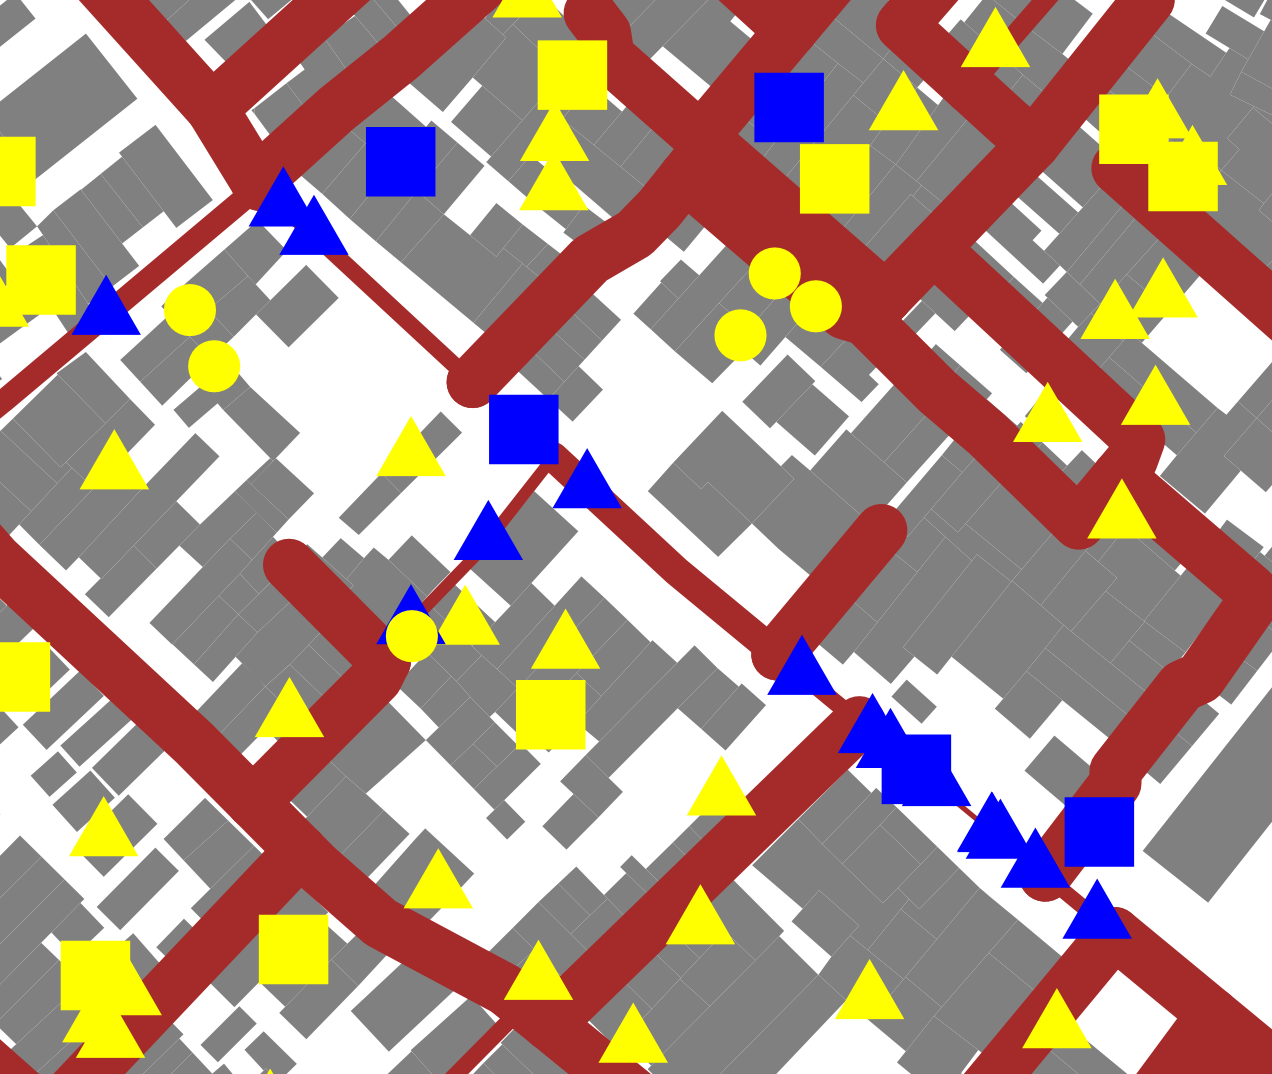
\includegraphics[width=0.6\textwidth]{../images/mobilities.png}
    \caption{Different mobilities of the inhabitant agents: Car (Square), Motorcycle (Triangle), Walking (Circle). Colors represent the evacuate status: Blue (Evacuating/Informed), Yellow (Uninformed).}
    \label{fig:mobilities}
\end{figure}

\subsection{Parameters}

The parameters of the simulation are set as follows (Fig \ref{fig:parameters}):
\begin{itemize}
    \item \textbf{Inform Strategy}: one of \{random, furthest, closest\}
    \item \textbf{Number of People}: default 1000
    \item \textbf{Alert Time}: the time before the tsunami arrives, default 120 minutes.
\end{itemize}

\begin{figure}
    \centering
    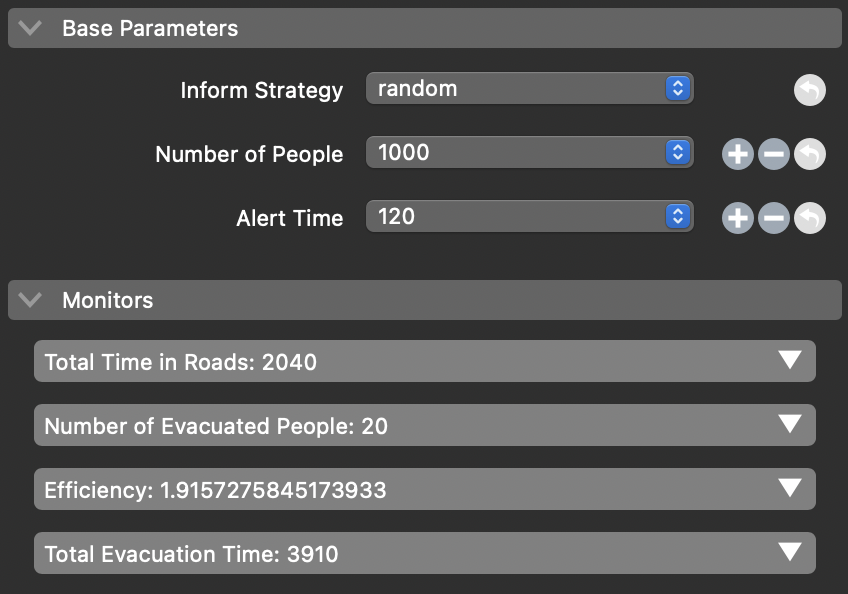
\includegraphics[width=0.6\textwidth]{../images/parameters.png}
    \caption{Parameters and Metrics of the simulation.}
    \label{fig:parameters}
\end{figure}

\subsection{Metrics}

To monitor and evaluate the evacuation process, I define the following metrics:
\begin{itemize}
    \item \textbf{Number of Evacuated People}: The number of people who have evacuated to the shelter before the tsunami arrives.
    \item \textbf{Total Time in Roads}: The total time people spend wandering on the roads to inform others and search for the shelter. To be specified, the time is counted from the time the inhabitant is informed and start evacuating until they reach the shelter.
    \item \textbf{Total Evacuation Time}: The time from the alert time until the last inhabitant evacuates to the shelter.
    \item \textbf{Efficiency}: The efficiency of the strategy.
\end{itemize}

The \textbf{Total Time in Roads} can be calculated by the formula:
\begin{align*}
    \text{Total Time in Roads} = \sum_{i=1}^{N} \text{T\_roads}_i
\end{align*}
\begin{align*}
    \text{T\_roads}_i = 
    \begin{cases}
        \text{t\_evacuated}_i - \text{t\_informed}_i & \text{if the inhabitant reaches the shelter} \\
        \text{t\_current} - \text{t\_informed}_i & \text{if the inhabitant is still on the road}
    \end{cases}
\end{align*}
where $\text{t\_evacuated}_i$ is the time the inhabitant $i$ reaches the shelter and $\text{t\_informed}_i$ is the time the inhabitant $i$ is informed and start evacuating, and N is the total of informed people. \\

The topic suggests the \textbf{Efficiency} of the strategy, which can be calculated by the formula:
\begin{align*}
    \text{Efficiency} = \frac{\text{Total Evacuation Time}}{\text{Total Time in Roads}}
\end{align*}

But after conducting the simulation, I found that this is not a good metric to evaluate the strategy. In the worst case, when the simulation stops because of running out of time, the total evacuation time equals the total simulation runtime, the total time spent on the roads could still be low if only 10\% of people were informed initially and went directly to the shelter without informing others. This scenario would yield a highest efficiency number despite being the worst strategy.\\

To correct this, I suggest the \textbf{Efficiency} metric to be calculated by the formula:
\begin{align*}
    \text{Efficiency} = \frac{\text{Total Evacuated people} \times \text{Alert Time}}{\text{Total Time in Roads} + 1}
\end{align*}

This metric will give a better evaluation of the strategy, as it tries to minimize the time people spend wandering on the roads to inform others and search for the shelter, and maximize the number of people informed, resulting in the total number of people evacuated. The $\text{+1}$ is added to avoid the division by zero. The scaling of the $\text{Alert Time}$ is added to make the division to be in the same unit.\\

Note that the chance of people successfully finding the shelter is random, and can't be controlled by the strategy. \textbf{The strategy only affects the number of people informed and the time they spend wandering on the roads, which possibility increases the chance of successfully evacuated people}.\\

\subsection{Results}

In this experiments, I conducted the simulation with different strategies and alert times. I also made the comparison between the different strategies by running them in parallel. About the map, I used the map of \textbf{Hanoi and the Red River} in the previous exercises. The shelter in this map is the one in the right-bottom corner (colored in green in the Fig \ref{fig:map}).\\ 

However, this building is too far from the others, which makes the evacuation process more difficult, since it's hard to people to realize it at distance 20m while wandering around. I made a change by selecting the building in the center-bottom of the map as the shelter. It is presented in red color in the Fig \ref{fig:map}. A quick experiment showed that in the settings of 3000 people and 2 hours of alert time, the number of evacuated people is increased to 298 compared to 248 of the previous shelter. Since the new shelter is more accessible, the results of comparison between the strategies are more reliable, as they eliminate the luck factor involved in finding the shelter and focus on the efficiency of the strategies.\\

\begin{figure}
    \centering
    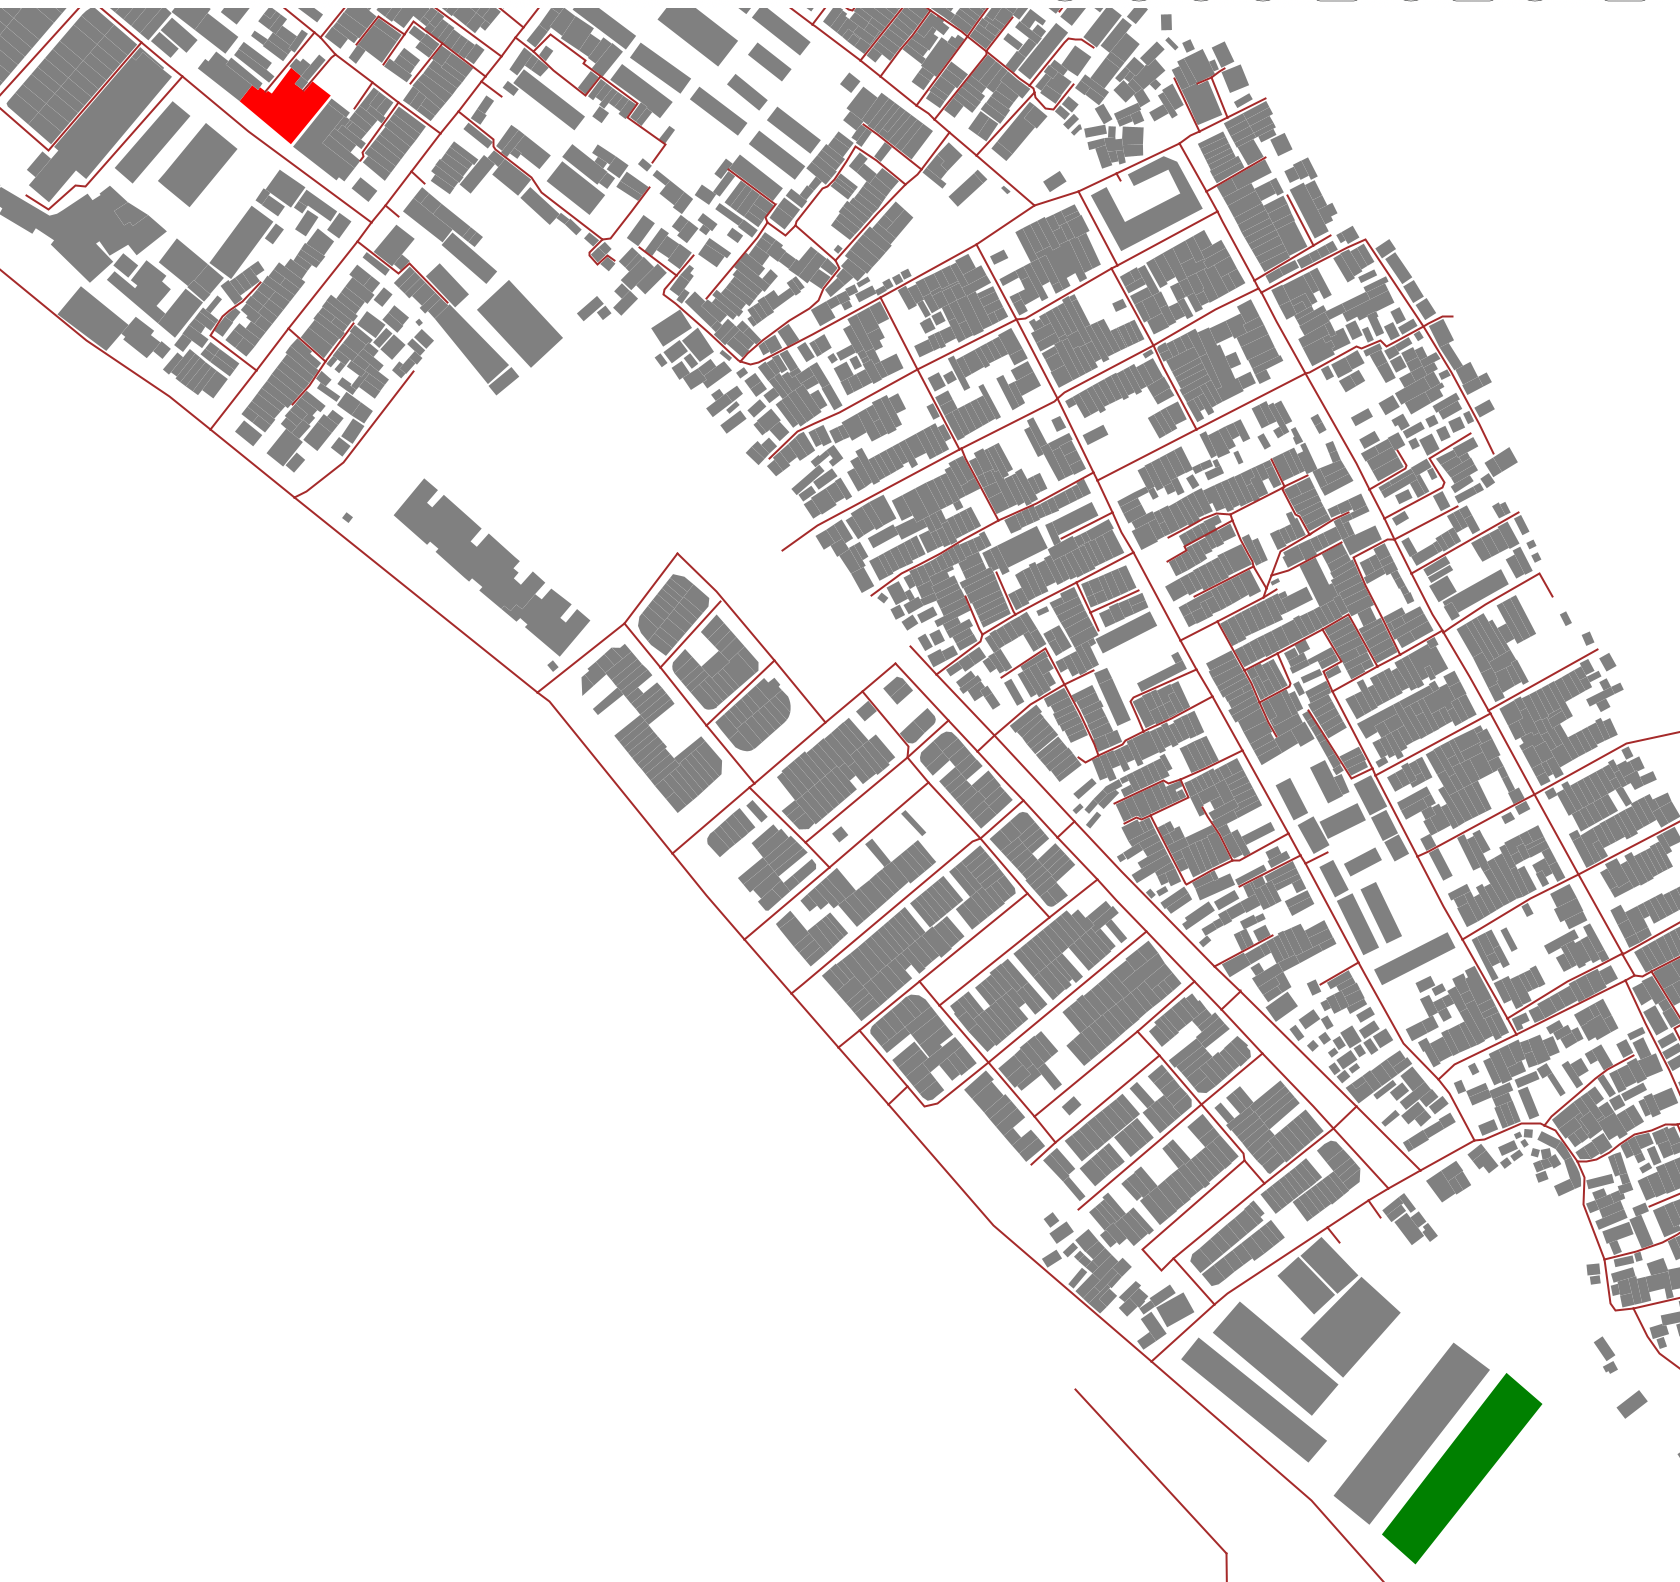
\includegraphics[width=0.6\textwidth]{../images/map0.png}
    \caption{The GIS data of Hanoi and the Red River. The largest building is in the bottom-right corner (colored in green). The shelter is in the center of the map (colored in red).}
    \label{fig:map}
\end{figure}

A single simulation of the evacuation process is presented in the Fig \ref{fig:results-single}. \\

The comparison of the different strategies in number of evacuated people is presented in the Fig \ref{fig:evacuees_over_time}. The experiment is conducted with 2000 and 4000 people, 2 hours alert time among the different strategies. The results show that, at the settings of large number of people, the \textbf{closest} strategy is the one that save the most people, followed by the \textbf{furthest} strategy, and the \textbf{random} strategy is the least efficient. At smaller number of people, the three strategies have similar results. In all cases, the \textbf{random} strategy introduces the fastest evacuation process at the beginning. These findings can be explained by some reasons:
\begin{itemize}
    \item The \textbf{random} strategy is the fastest at the beginning because the people are randomly selected, which means they are distributed evenly across the map, so the people can start finding the shelter from diverse locations, which reduces the traffic congestion and the time people spend wandering on the roads, but the chance of people finding the shelter isn't increased.
    \item The \textbf{closest} strategy introduces the largest number of people saved because the people closest to the shelter have chance to inform others closed to the shelter as well, which increases the chance of people finding the shelter.
\end{itemize}

Next, I conducted the batch exploration to examine which strategy is the most efficient, which determined in the previous section. The results are presented in the Fig \ref{fig:batch}.


\begin{figure}
    \centering
    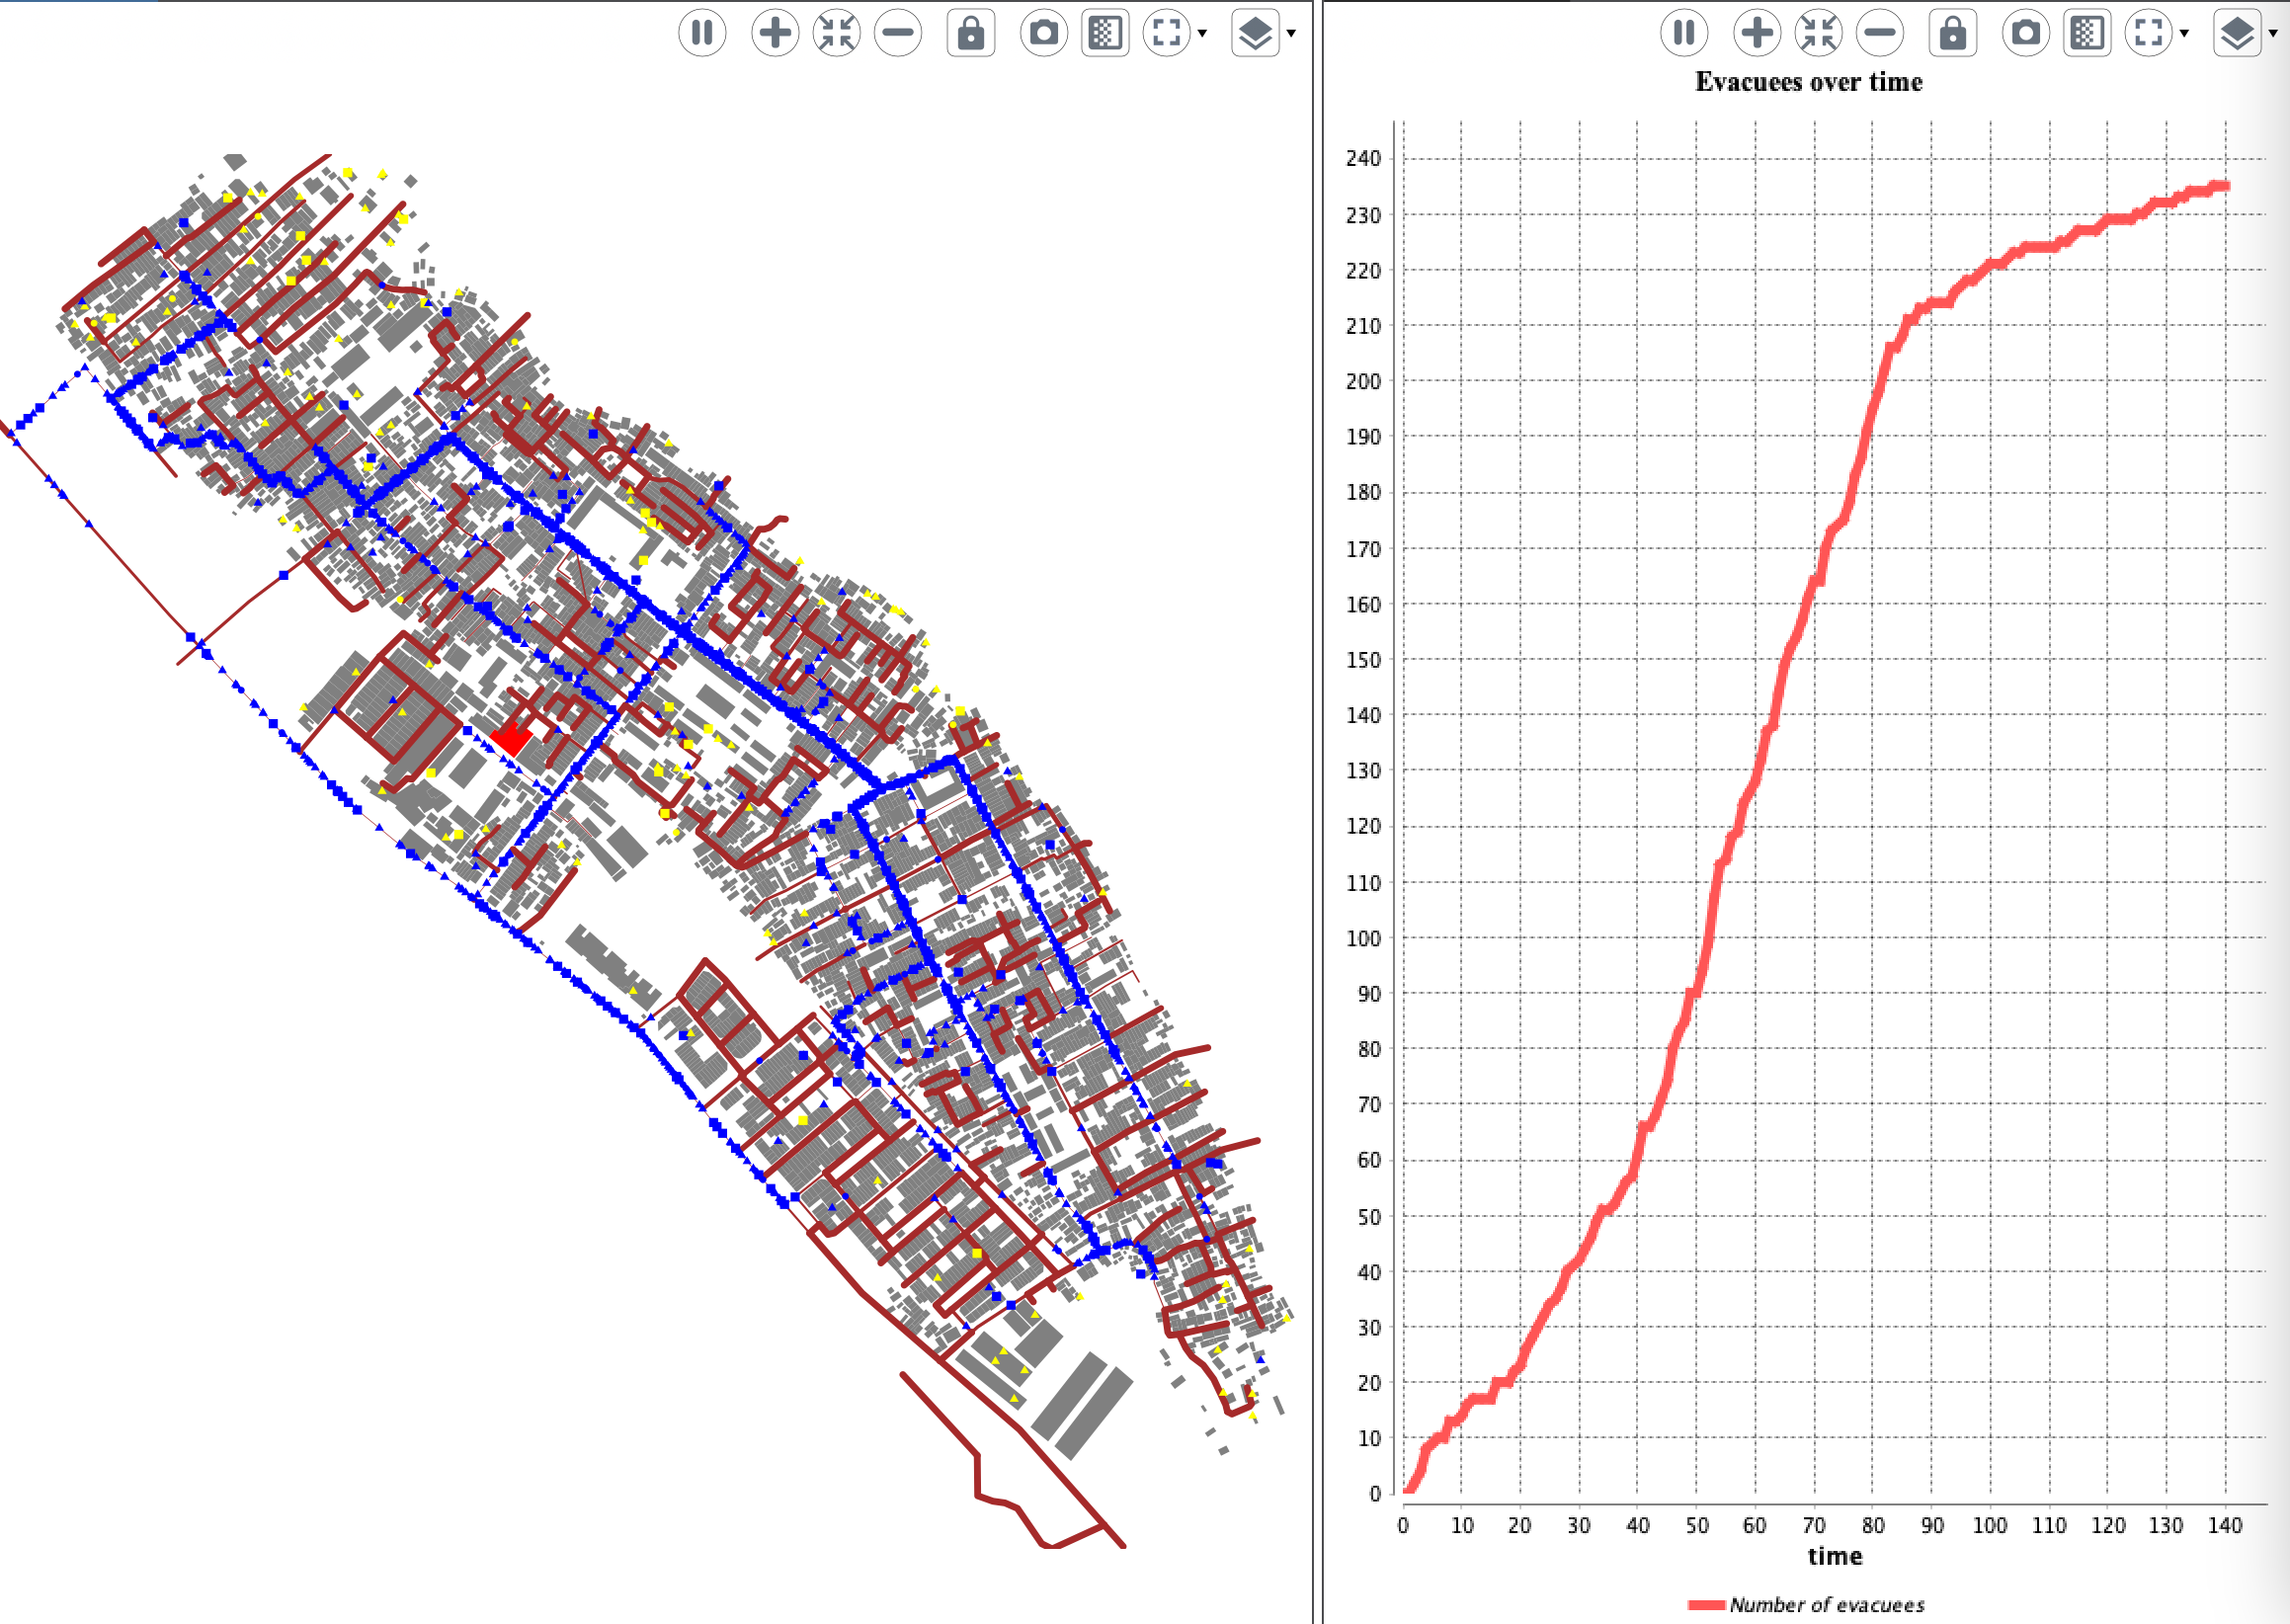
\includegraphics[width=0.8\textwidth]{../images/single-simulation.png}
    \caption{The evacuation simulation with 1000 people, \textbf{random} strategy and 2 hours evacuate time. The right chart is the total number of evacuated people over time. The red building in the right-bottom corner is the shelter.}
    \label{fig:results-single}
\end{figure}

\begin{figure}
    \centering
    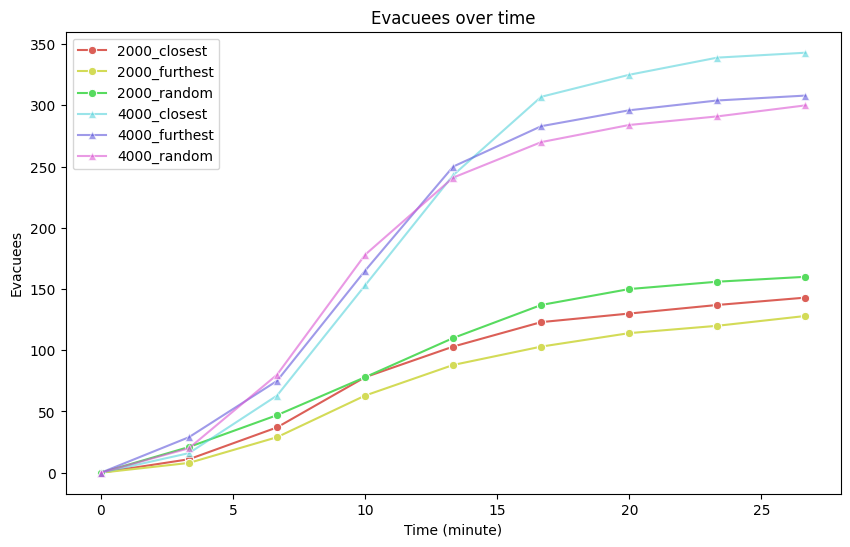
\includegraphics[width=0.8\textwidth]{../images/evacuees_over_time.png}
    \caption{The comparison of the different strategies in number of evacuated people over time.}
    \label{fig:evacuees_over_time}
\end{figure}

% --------------------------
% 4. Discussion
% --------------------------
\section{Discussion}


% --------------------------
% 4. Discussion
% --------------------------
\section*{Appendix A}


\section{General Information}
\subsection{What is the title of the project?}

\begin{examplebox}
Evaluating methods for the analysis of pre--post measurement experiments
\end{examplebox}

\textit{Answer:}

\subsection{Who are the current and future project contributors?}

\begin{examplebox}
    Björn S. Siepe, František Bartoš, and Samuel Pawel
\end{examplebox}

\textit{Answer:}

\subsection{Provide a description of the project.}

\explanation{This can also include empirical examples that will be analyzed within the same project, especially if the analysis depends on the results of the simulation.} 

\begin{examplebox}
    We will investigate the performance of different methods for analyzing data from pre--post measurement experiments. We will conduct a single simulation study varying the treatment effect and the pre--post measure correlation. We will compare three different methods (ANCOVA, change score analysis, and post score analysis) using power and type I error rate related to the hypothesis test of no effect, and bias related to the effect estimate (in an actual simulation study aimed at evaluating estimation of the effect size, a performance measure assessing variance, i.e., empirical standard error, would be also recommended).  
\end{examplebox}

\textit{Answer:}

\subsection{Did any of the contributors already conduct related simulation studies on this specific question?}

\explanation{This includes preliminary simulations in the context of the current project.} 

\begin{examplebox}
    We did not conduct previous simulation studies for pre--post measurement experiments but we were inspired by the previous literature on the topic \parencite{vickers2001use, senn2006change, van2013ancova, clifton2019correlation, ludtke2023ancova}.
\end{examplebox}

\textit{Answer:}

\section{Aims}
\subsection{What is the aim of the simulation study?}
 
\explanation{The aim of a simulation study refers to the goal of the research and shapes subsequent choices. Aims are typically related to evaluating the properties of a method (or multiple methods) with respect to a particular statistical task. Possible tasks include `estimation', `hypothesis testing', `model selection', `prediction', or `design'. If possible, try to be specific and not merely state that the aim is to `investigate the performance of method \textit{X} under different circumstances'.} 
    
\begin{examplebox}
The aim of the simulation study is to evaluate different methods for analyzing data from pre--post measurement experiments with respect to their hypothesis testing and estimation characteristics.
\end{examplebox}

\textit{Answer:}


\section{Data-Generating Mechanism}
\subsection{How will the parameters for the data-generating mechanism (DGM) be specified?}

\explanation{Answers include `parametric based on real data', `parametric', or `resampled'. Parametric based on real data usually refers to fitting a model to real data and using the parameters of that model to simulate new data. Parametric refers to generating data from a known model or distribution, which may be specified based on theoretical or statistical knowledge, intuition, or to test extreme values. Resampled refers to resampling data from a certain data set, in which case the true data-generating mechanism is unknown. The answer to this question may include an explanation of from which distributions (with which parameters) values are drawn, or code used to generate parameter values. If the DGM parameters are based on real data, please provide information on the data set they are based on and the model used to obtain the parameters. Also, indicate if any of the authors are already familiar with the data set, e.g., analyzed (a subset of) it.} 
    
\begin{examplebox}
In each simulation repetition, we generate $n=50$ pre--post measurements in the control group ($g = \text{control}$) and $n = 50$ pre--post measurements in the experimental group ($g = \text{exp}$) from a bivariate normal distribution
\begin{equation}
    \label{eq:bivariateNormal}
    \left[\begin{array}{c}Y_1 \\ Y_2 \end{array}\right] \sim\text{N}\left(\left[\begin{array}{c}0 \\ \mu_{g,2} \end{array}\right],\left[\begin{array}{cc} 1 & \rho  \\ \rho & 1 \end{array}\right]\right),
\end{equation}
where the first argument of the normal distribution is the mean vector and the second argument the covariance matrix.
The numerical subscript 1 indicates measurement time `pre' and 2 indicates `post'. The parameter $\mu_{g,2}$ denotes the post-treatment mean. It is fixed to zero in the control group (${\mu_{\text{control},2}} = 0$), whereas it is varied across simulation conditions in the experimental group. The parameter $\rho$ denotes the pre--post correlation and is also varied across simulation conditions. 
\end{examplebox}

\textit{Answer:}

\subsection{What will be the different factors of the data-generating mechanism?} 

\explanation{A factor can be a parameter/setting/process/etc. that determines the data-generating mechanism and is varied across simulation conditions.}

\begin{examplebox}
We will vary the following factors:
\begin{itemize}
    \item the post-treatment mean in the experimental condition ${\mu_{\text{exp},2}}$
    \item the pre--post measurement correlation $\rho$
\end{itemize}
\end{examplebox}

\textit{Answer:}
    
\subsection{If possible, provide specific factor values for the DGM as well as additional simulation settings.} 

\explanation{Also include information about settings that are held constant across simulation conditions. This may include a justification of the chosen values and settings.}
    
\begin{examplebox}
We will use the following values for our data-generating mechanism:
\begin{itemize}
        \item ${\mu_{\text{exp},2}} \in \{0, 0.2, 0.5\}$
        \item $\rho \in \{0, 0.5, 0.7\}$
\end{itemize}
We selected these specific values for the post-treatment mean in the experimental condition as they correspond to the conventions for no, small, and medium standardized mean difference effect sizes in psychology \parencite{Cohen1988} and pre--post measurement correlations that correspond to no, one quarter, and approximately one half of the shared variance. Based on our experience, these parameter values are relevant for empirical research while covering a sufficiently large range to allow us to observe possible differences between the examined methods. For simplicity of the example, we consider only a single sample size, namely, $n = 50$ per group.
\end{examplebox}

\textit{Answer:}

\subsection{If there is more than one factor: How will the factor levels be combined and how many simulation conditions will this create?} 

\explanation{Answers include `fully factorial', `partially factorial', `one-at-a-time', or `scattershot'. Fully factorial designs are designs in which all possible factor combinations are considered. Partially factorial designs denote designs in which only a subset of all possible factor combinations are used. One-at-a-time designs are designs where each factor is varied while the others are kept fixed at a certain value. Scattershot designs include distinct scenarios, for example, based on parameter values from real-world data.} 
    
\begin{examplebox}
We will vary the conditions in a fully factorial manner. This will result in\\ \mbox{3 (post-treatment mean in experimental group)} $\times$ 3 (pre--post measurement correlation) = 9 simulation conditions.
\end{examplebox} 

\textit{Answer:}


\section{Estimands and Targets}
\subsection{What will be the estimands and/or targets of the simulation study?}      

\explanation{Estimands and other targets jointly refer to the practical aims of the compared methods. For example, an estimand/target could be the true effect size estimated by the compared methods \parencite[see][for more information]{Siepe2024}. Please also specify if some targets are considered more important than others, i.e., if the simulation study will have primary and secondary outcomes.} 
    
\begin{examplebox}
Our primary target is the null hypothesis of no difference between the outcomes of the control and treatment groups. Our secondary estimand is the treatment effect size defined as the expected difference between the control and the experimental group measurements at time-point two
\begin{align*}
    \text{E}(Y_2 \mid g=\text{exp}) - \text{E}(Y_2 \mid g=\text{control}),
\end{align*}
for which the true value is given by the parameter $\mu_{\text{exp},2}$ for the considered data-generating mechanisms. 
\end{examplebox}  

\textit{Answer:}

\section{Methods}
\subsection{How many and which methods will be included and which quantities will be extracted?}
    
\explanation{Be as specific as possible regarding the methods that will be compared, and provide a justification for both the choice of methods and their model parameters. This can also include code which will be used to estimate the different methods or models in the simulation with all relevant model parameters. Setting different prior hyperparameters might also be regarded as using different methods. Where package defaults are used, state this. Where they are not used, state what values are used instead.}

\begin{examplebox}
We will compare the following methods:
    \begin{itemize}
    \item[1)] \textbf{ANCOVA} (ANalysis of COVAriance): A regression of the post-treatment measurement using the pre-treatment measurement and the treatment indicator as covariates,
    which is specified in R as 
    \begin{verbatim}
        lm(post ~ pre + treatment)
    \end{verbatim}
        
    \item[2)] \textbf{Change score analysis}: A regression of the difference between post-treatment and pre-treatment measurement using the treatment indicator as covariate,
    which is specified in R as 
    \begin{verbatim}
        lm(post ~ offset(pre) + treatment)
    \end{verbatim}
        
    \item[3)] \textbf{Post score analysis}: A regression of the post-treatment measurement using the treatment indicator as covariate,
    which is specified in R as 
    \begin{verbatim}
        lm(post ~ treatment)
    \end{verbatim}
\end{itemize}
Both change score and post score ANOVA can be seen as a special case of ANCOVA. Change score analysis fixes the \texttt{pre} coefficient to 1 (using the \texttt{offset()} function) and post score analysis omits the \texttt{pre} variable from the model (effectively fixing its coefficient to 0).

From each fitted model, we will extract the estimated treatment effect, the associated standard error, and the associated two-sided $t$-test \textit{p}-value for the null hypothesis of no effect. A rejection of the null hypothesis will be defined by a \textit{p}-value less than the conventional threshold of 0.05.
\end{examplebox} 

\textit{Answer:}

\section{Performance Measures}
\subsection{Which performance measures will be used?}    

\explanation{Please provide details on why they were chosen and on how these measures will be calculated. Ideally, provide formulas for the performance measures to avoid ambiguity. Some models in psychology, such as item response theory or time series models, often contain multiple parameters of interest, and their number may vary across conditions. With a large number of estimated parameters, their performance measures are often combined. If multiple estimates are aggregated, specify how this aggregation will be performed. For example, if there are multiple parameters in a particular condition, the mean of the individual biases of these parameters or the bias of each individual parameter may be reported.}  
    
\begin{examplebox}
Our primary performance measures are the type I error rate (in conditions where the true effect is zero) and the power (in conditions where the true effect is non-zero) to reject the null hypothesis of no difference between the control and treatment condition. The null hypothesis is rejected if the \textit{p}-value for the null hypothesis of no effect is less than or equal to the conventional threshold of 0.05. The rejection rate (the type I error rate or the power, depending on the data generating mechanism) is estimated by 
\begin{align*}
   \widehat{\text{RRate}} = \frac{\sum_{i=1}^{n_{\text{sim}}} 1(p_i \leq 0.05)}{n_{\text{sim}}}
\end{align*}
where $1(p_i \leq 0.05)$ is the indicator of whether the \textit{p}-value in simulation $i$ is equal to or less than 0.05. We use the following formula to compute the MCSE of the rejection rate
\begin{align*}
    \text{MCSE}_{\widehat{\text{RRate}}} = \sqrt{\frac{\widehat{\text{RRate}} (1 - \widehat{\text{RRate}})}{n_{\text{sim}}}}.
\end{align*}
Our secondary performance measure is the bias of the treatment effect estimate. It is estimated by 
\begin{align*}
   \widehat{\text{Bias}} = \frac{\sum_{i=1}^{n_{\text{sim}}} \hat{\theta}_i}{n_{\text{sim}}} - \theta
\end{align*}
where $\theta$ is the true treatment effect and $\hat{\theta}_i$ is the effect estimate from simulation $i$. We compute the MCSE of the estimated bias with
\begin{align*}
    \text{MCSE}_{\widehat{\text{Bias}}} = \frac{S_{\hat{\theta}}}{\sqrt{n_{\text{sim}}}}
\end{align*}
where $S_{\hat{\theta}} = \sqrt{\sum_{i=1}^{n_{\text{sim}}}{ \{\hat{\theta}_i - (\sum_{i=1}^{n_{\text{sim}}}\hat{\theta}_i/n_{\text{sim}})\}^2}/(n_{\text{sim}} - 1)}$ is the sample standard deviation of the effect estimates.
\end{examplebox}

\textit{Answer:}

\subsection{How will Monte Carlo uncertainty of the estimated performance measures be calculated and reported?} 
    
\explanation{Ideally, Monte Carlo uncertainty can be reported in the form of Monte Carlo Standard Errors (MCSEs). Please see \textcite{Siepe2024} and \textcite{Morris2019} for a list of formulae to calculate the MCSE related to common performance measures, more accurate jackknife-based MCSEs are available through the \texttt{rsimsum} \parencite{Gasparini2018} and \texttt{simhelpers} \parencite{Simhelpers2022} R packages, the \texttt{SimDesign} \parencite{Chalmers2020} R package can compute confidence intervals for performance measures via bootstrapping. Monte Carlo uncertainty can additionally be visualized using plots appropriate for illustrating variability, such as MCSE error bars, histograms, boxplots, or violin plots of performance measure estimates, if possible (e.g., bias).}
    
\begin{examplebox}
We will report Monte Carlo uncertainty in tables (MCSEs next to the estimated performance measures) and in plots (error bars with $\pm 1$MCSE around estimated performance measures). We will use the formulas provided in \textcite{Siepe2024} to calculate MCSEs, see our answer to the last question.
\end{examplebox}

\textit{Answer:}
   
\subsection{How many simulation repetitions will be used for each condition?}  

\explanation{Please also indicate whether the chosen number of simulation repetitions is based on sample size calculations, on computational constraints, rules of thumb, or any other heuristic or combination of these strategies. Formulas for sample size planning in simulation studies are provided in \textcite{Siepe2024}. If there is a lack of knowledge on a quantity for computing the Monte Carlo standard error (MCSE) of an estimated performance measure (e.g., the variance of the estimator is needed to compute the MCSE for the bias), pilot simulations may be needed to obtain a guess for realistic/worst-case values.}
    
\begin{examplebox}
We will perform 10,000 repetitions per condition. We determined this number by aiming for a MCSE of 0.005 for the type I error rate and the power under the ``worst-case'' rejection rate of 50\% in the sense that the MCSE is maximal for a given number of repetitions ($0.50 \times (1 - 0.50) / 0.005^2 = 10{,}000$ repetitions).
    
For illustration, we also determined the required number of repetitions to achieve a MCSE of 0.005 for the bias for each of the methods. The sample size calculation requires the empirical variance of the effect estimates $S_{\hat{\theta}}^2$ for each method. Since the empirical variances of the effect estimates can vary (pun intended) across simulation conditions, we compute the sample size using the largest estimated variance across all conditions. We obtain the empirical variance estimates for each condition and method using 100 pilot simulation runs. We found that the required sample sizes would be $S_{\hat{\theta}}^2/0.005^2 = 1{,}986$ for ANCOVA, $S_{\hat{\theta}}^2/0.005^2 = 3{,}812$ for change score analysis, and $S_{\hat{\theta}}^2/0.005^2 = 1{,}996$ for post score analysis.
\end{examplebox}

\textit{Answer:}




\subsection{How will missing values due to non-convergence or other reasons be handled?}
    
\explanation{`Convergence' means that a method successfully produces the outcomes of interest (e.g., an estimate, a prediction, a \textit{p}-value, a sample size, etc.) that are required for estimating the performance measures. Non-convergence of some repetitions or whole conditions of simulation studies occurs regularly, e.g., for numerical reasons. It is possible to impute non-converged repetitions, exclude all non-converged repetitions or to implement mechanisms that repeat certain parts of the simulation (such as data generation or model fitting) until convergence is achieved. Further, it is important to consider at which proportion of failed repetitions a whole condition will be excluded from the analysis. See \textcite{Pawel2024} for more guidance on handling missing values in simulation studies.}
    
\begin{examplebox}
We do not expect missing values or non-convergence. If we observe any non-convergence, we exclude the non-converged cases case-wise (keeping the converged values from the other methods in the same repetition) and report the number of non-converged cases per method and condition.
\end{examplebox} 

\textit{Answer:}

\subsection{How do you plan on interpreting the performance measures? \textmd{(optional)}}
    
\explanation{It can be specified what a `relevant difference' in performance, or what `acceptable' and `unacceptable' levels of performance might be to avoid post-hoc interpretation of performance. Furthermore, some researchers use regression models to analyze the results of simulations and compute effect sizes for different factors, or to assess the strength of evidence for the influence of a certain factor \parencite{Skrondal2000, Chipman2022}. If such an approach will be used, please provide as many details as possible on the planned analyses.}
    
\begin{examplebox}
We define a type I error rate larger than 5\% as non-acceptable performance. Amongst methods that exhibit acceptable performance regarding the type I error rate (within the MCSE), we consider a method X as performing better than a method Y in a certain simulation condition if the lower bound for the estimated power of method X ($\widehat{\text{Pow}}-\text{MCSE}$) is greater than the upper bound for the estimated power of method Y ($\widehat{\text{Pow}}+\text{MCSE}$).
\end{examplebox} 

\textit{Answer:}

\section{Other}
\subsection{Which statistical software/packages do you plan to use?}   

\explanation{Likely, not all software used can be prespecified before conducting the simulation. However, the main packages used for model fitting are usually known in advance and can be listed here, ideally with version numbers.} 
    
\begin{examplebox}
We will use the following packages of \texttt{R} version 4.3.1 \parencite{R2020} in their most recent versions: The \texttt{mvtnorm} package \parencite{Genz2009} to generate data, the \texttt{lm()} function included in the \texttt{stats} package \parencite{R2020} to fit the different models, the \texttt{SimDesign} package \parencite{Chalmers2020} to set up  and run the simulation study, and the \texttt{ggplot2} package \parencite{Wickham2016} to create visualizations.  
\end{examplebox}

\textit{Answer:}

\subsection{Which computational environment do you plan to use?} 
    
\explanation{Please specify the operating system and its version which you intend to use. If the study is performed on multiple machines or servers, provide information for each one of them, if possible.}
    
\begin{examplebox}
We will run the simulation study on a Windows 11 machine. The complete output of \texttt{sessionInfo()} will be saved and reported in the supplementary materials.
\end{examplebox}

\textit{Answer:}

\subsection{Which other steps will you undertake to make simulation results reproducible? \textmd{(optional)}} 
    
\explanation{This can include sharing the code and full or intermediate results of the simulation in an open online repository. Additionally, this may include supplemental materials or interactive data visualizations, such as a shiny application.}
    
\begin{examplebox}
We will upload the fully reproducible simulation script and a data set containing all relevant estimates, standard errors, and \textit{p}-values for each repetition of the simulation to OSF (\url{https://osf.io/dfgvu/}) and GitHub (\url{https://github.com/bsiepe/SimPsychReview}). 
\end{examplebox}

\textit{Answer:}

\subsection{Is there anything else you want to preregister? \textmd{(optional)}}
    
\explanation{For example, the answer could include the most likely obstacles in the simulation design, and the plans to overcome them, or measures that increase the trust in the preregistration date (e.g., setting the seed based on a future event), as explained in the introduction of this template.}
    
\begin{examplebox}
No.
\end{examplebox} 

\textit{Answer:}

\newpage
\section*{References}
\nocite{Siepe2024}
\printbibliography[heading=none]

\end{document}
